%************************************************
\chapter*{Introducción}\label{ch:introduccion}
%************************************************

El término Internet de las Cosas, o \textit{Internet of Things} (IoT) en inglés, tiene un amplio rango de interpretaciones \citep{Atzori20102787}, pero podemos resumirlo en miles de millones de dispositivos, en su mayoría de capacidad computacional limitada, que están interconectados entre sí e Internet, a fin de realizar algún objetivo común. Por ejemplo, una red de farolas en una calle de la ciudad, donde cada farola tiene un sensor de proximidad, y se comunica con las siguientes farolas para iluminar antes la calle, mejorando la seguridad y ahorrando energía; invernaderos con riego automatizado en base a los sensores de humedad repartidos por la tierra, mejorando la calidad de la plantación, y ahorrando agua; coches comunicándose entre sí para dar aviso de accidentes a los que vienen detrás, o indicando rutas alternativas para minimizar los atascos y la contaminación dentro de la ciudad. 


Muchos de estos objetivos requieren recopilar una gran cantidad de datos por medio de sensores, y gracias a organizaciones como \href{https://wikileaks.org/}{WikiLeaks}, los usuarios son cada vez más conscientes de la implicación que suponen sus datos en Internet, y demandan más seguridad y privacidad para ellos. Esto incluye tanto los datos que los usuarios comparten, sino también los datos recopilados sobre nosotros y sobre los que no tenemos un control directo. El ataque informático sufrido por Sony en 2011\footnote{2011 PlayStation Network outage - 
\url{https://en.wikipedia.org/wiki/2011_PlayStation_Network_outage}} afectó a su red de jugadores de consola, cuya información de facturación estaba guardada en sus servidores, y debido a que dicha información dependía tanto de los usuarios como de Sony para estar segura, aunque los usuarios la protegieran, se vieron comprometidos igualmente.

In traditional M2M (Machine to Machine) environments the issues about security and privacy have already been treated deeply, but in the IoT world, due to it's recent and fast growth, lacks of those tools to solve autonomously these problems.

En entornos tradicionales, los problemas de seguridad y privacidad ya han sido tratados en profundidad, pero en el mundo de IoT, debido a su reciente y rápido crecimiento, carece de esas herramientas para resolver estos problemas.

Con la proliferación de dispositivos IoT recopilando tanta información como son capaces con sus sensores, la cantidad de datos recopilados sobre cualquier persona puede ser enorme. Y el IoT ha demostrado no ser de confianza para la seguridad ni la privacidad, como en el reciente ataque DDoS de la \textit{botnet} Mirai, en octubre de 2016, considerado el ataque DDoS más grande de la historia\citep{jeyanthi:2017}, o las múltiples vulnerabilidades descubiertas en aparatos del hogar, como monitores de bebé\citep{rapid7babycam}.

Para solucionar este problema de privacidad en Internet, aparece el concepto de \textit{anonimidad fuerte}, que oculta nuestros datos personales, pero que nos permite poder seguir operando en Internet como individuos independientes\citep{stronganonymity}. Para conseguir esto, debemos realizar los procesos de autenticación y autorización de la manera más privada posible. Las credenciales basadas en atributos y la \textit{selección selectiva} de los mismos, permite controlar qué información revelamos a terceros, bajo un sistema criptográfico de confianza para ambas partes.

Una credencial basada en atributos puede entenderse como una firma digital, realizada por un Emisor, sobre una lista de pares atributo-valor, por ej., la lista \texttt{\justify{(nombre=Alice, apellido=Anderson, fechaNac=1977-05-10, nacionalidad=DE)}}\citep{introCredIBM}.


El método más directo, como Usuario, para convencer a un Verificador de que se poseen los valores firmados en el certificado, sería simplemente enviar la credencial en claro, mostrando todos los atributos. Con credenciales anónimas, el Usuario nunca transmite la credencial en sí, sino que usa una criptografía especial para convencer al Verificador de que sus atributos cumplen alguna propiedad, sin mostrarlos directamente, por ejemplo, que la diferencia entre la fecha actual y la fecha de nacimiento en el certificado es mayor a 18 años. Una ventaja directa es que el Verificador no puede reutilizar esa prueba con terceras partes, pues no posee el certificado, lo que evita el robo de información.


Con la criptografía simétrica o asimétrica usual utilizada en los certificados más populares, como los TLS/SSL para las webs de Internet, no es posible llevar a cabo esas \textit{pruebas} sin una explosión combinatoria de firmas de certificados de todas las posibles pruebas a presentar. Las soluciones para la privacidad actuales utilizan las llamadas Pruebas de Conocimiento Cero (ZKP), cuya teoría estudio más en profundidad en mi TFG de Matemáticas\citep{tfgmates}, y en resumen, permiten demostrar conocimiento de algún dato secreto, sin revelar nada más que el hecho de conocer dicho dato, de ahí la parte de \textit{conocimiento cero}.

Para explicar brevemente cómo las ZKP funcionan, en 1990 Guillou, Quisquater y Berson publicaron \textit{How to Explain Zero-Knowledge Protocols to Your Children} \citep{ZKPcave:story}, una historia sobre cómo Alí Babá demostró que sabía las palabras mágicas para abrir la cueva, pero sin decirle a nadie dichas palabras. A continuación presentamos una versión reducida, pero que subraya las propiedades básicas de toda ZKP.

To understand how ZKPs work, in 1990 Guillou, Quisquater and Berson published in \textit{How to Explain Zero-Knowledge Protocols to Your Children} \citep{ZKPcave:story} a story about how Ali Baba proved that he knew the magic words to open the cave, but without revealing those words to anyone. Here we present a brief version highlighting the properties of ZKPs.

\hfil


\begin{quote}
	Imaginemos una cueva, donde el camino principal se bifurca y al final de cada pasillo los caminos se vuelven a encontrar, formando una especie de anillo. En el punto en que se unen, dentro de la cueva, hay una puerta mágica con una palabra secreta, la cual permite abrirla y cruzar al otro lado.
	
	\textbf{P}aula conoce la clave secreta y quiere \textbf{p}robarlo a su amigo Víctor, pero sin tener que revelársela.
	\marginpar{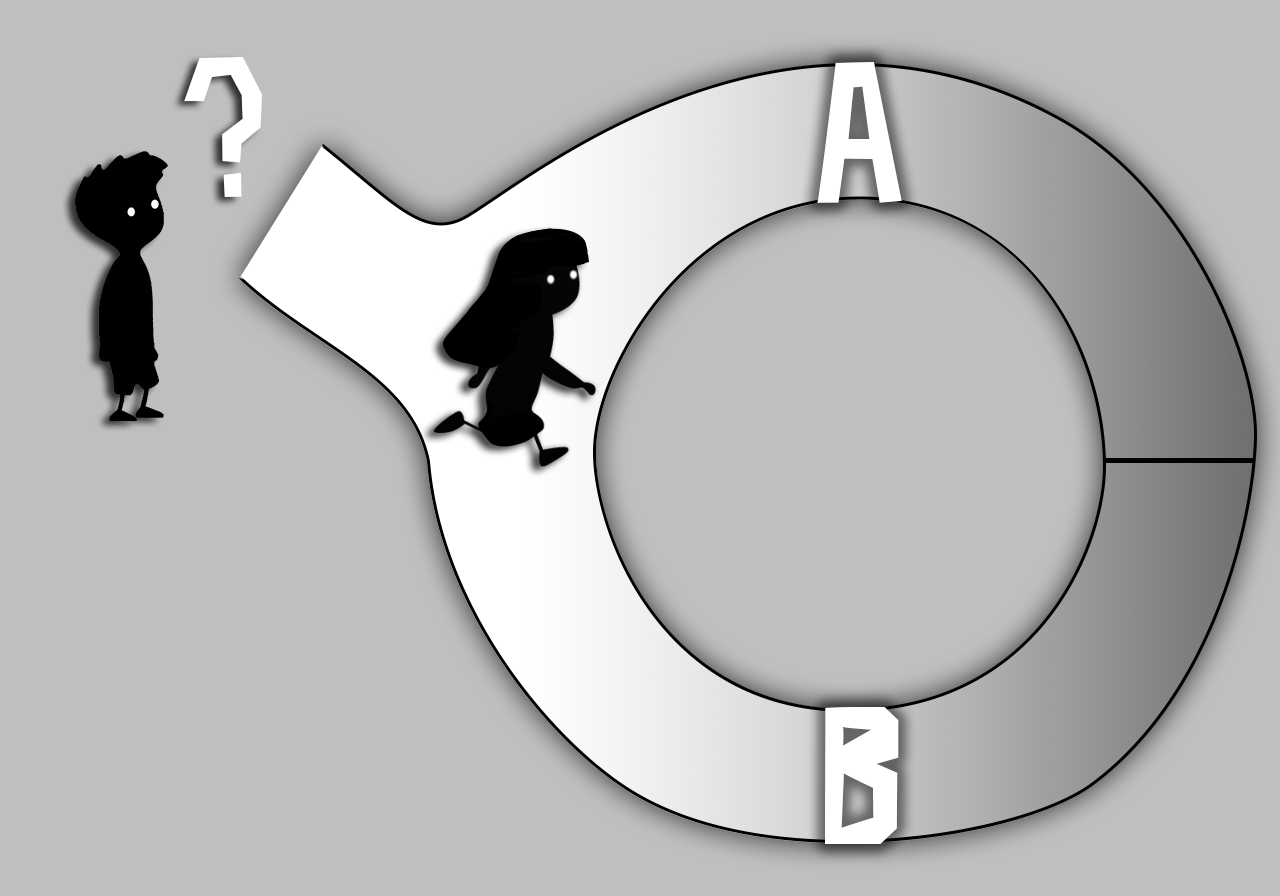
\includegraphics[width=1.\linewidth]{gfx/graficoJL_ZKP_1}\\La cueva \citep{ZKPcave:fig}
		. Paula entra por A o B al azar. Víctor espera fuera.}
	Paula y Víctor quedan en la entrada de la cueva con unos \textit{walkie-talkies}, de modo que Víctor esperará fuera y Paula entrará a la cueva y tomará uno de los pasillos, que llamaremos A y B, sin decirle cuál a Víctor.
	
	%\begin{figure}[bth]
	%	\begin{center}
	%		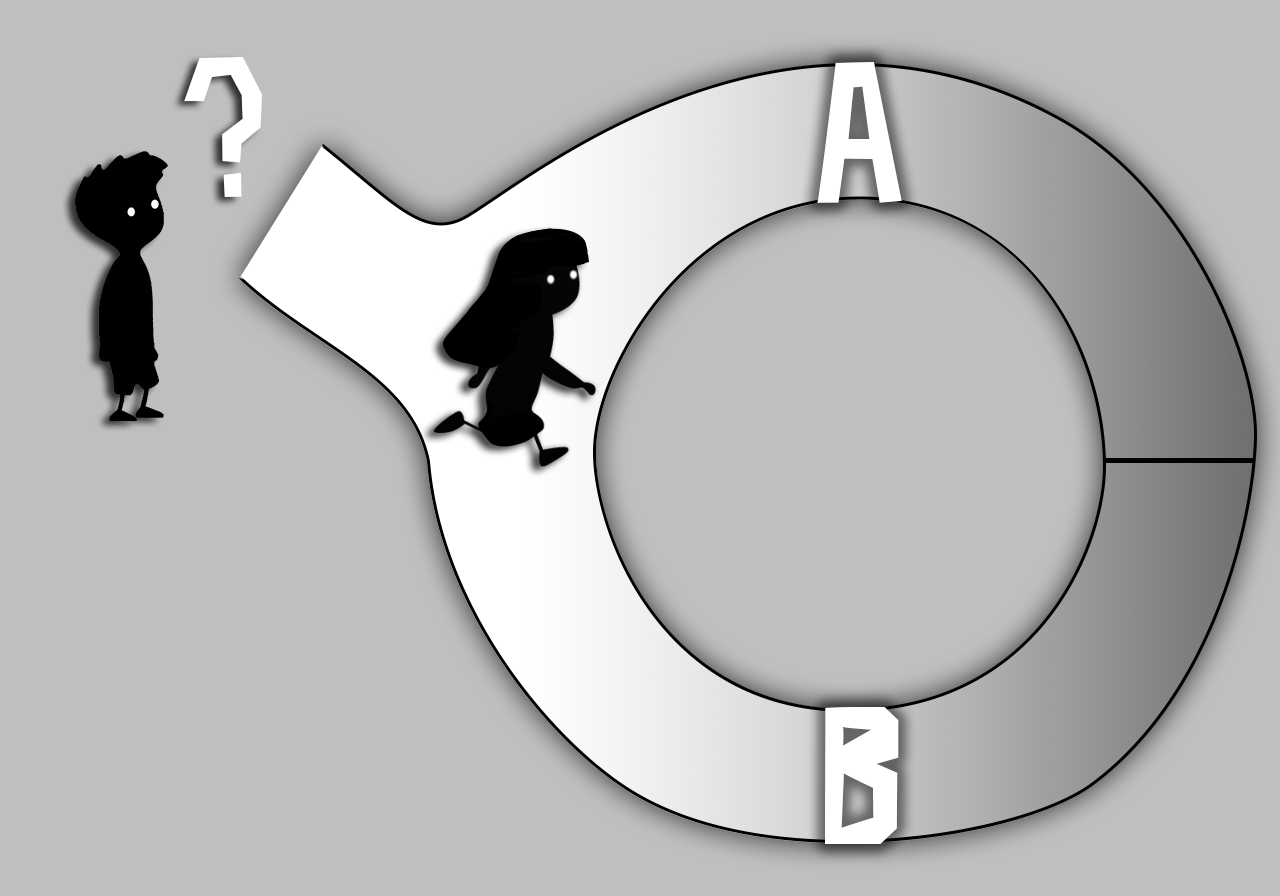
\includegraphics[width=.45\linewidth]{gfx/graficoJL_ZKP_1}
	%	\end{center}
	%	\caption{La cueva \citep{ZKPcave:fig}. Paula entra por A o B al azar, Víctor espera fuera.}
	%	\label{fig:ZKPcave1}
	%\end{figure}
	
	Al llegar a la puerta, Paula avisa a Víctor para que entre a la cueva y espere en la bifurcación, donde \textbf{V}íctor, para intentar \textbf{v}erificar que Paula conoce la palabra secreta, le indicará por qué pasillo quiere que vuelva, el A o el B.
	
	
	%\begin{figure}[bth]
	%	\begin{center}
	%		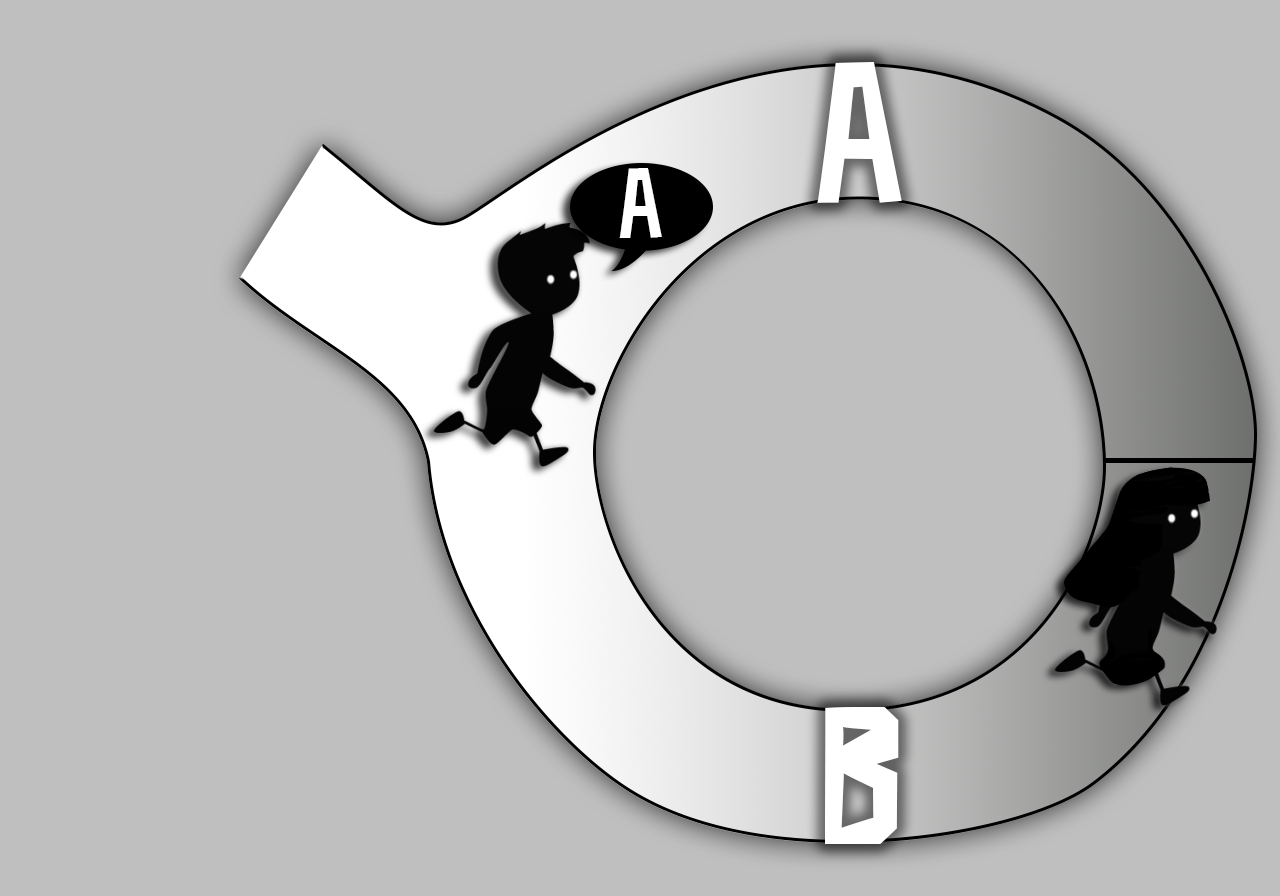
\includegraphics[width=.45\linewidth]{gfx/graficoJL_ZKP_2}
	%	\end{center}
	%	\caption{La cueva. Víctor elige al azar por dónde quiere que regrese Paula.}
	%	\label{fig:ZKPcave2}
	%\end{figure}
	
	Si Paula realmente conoce el secreto, podrá volver a la bifurcación por el pasillo solicitado, abriendo, si es preciso, la puerta.\marginpar{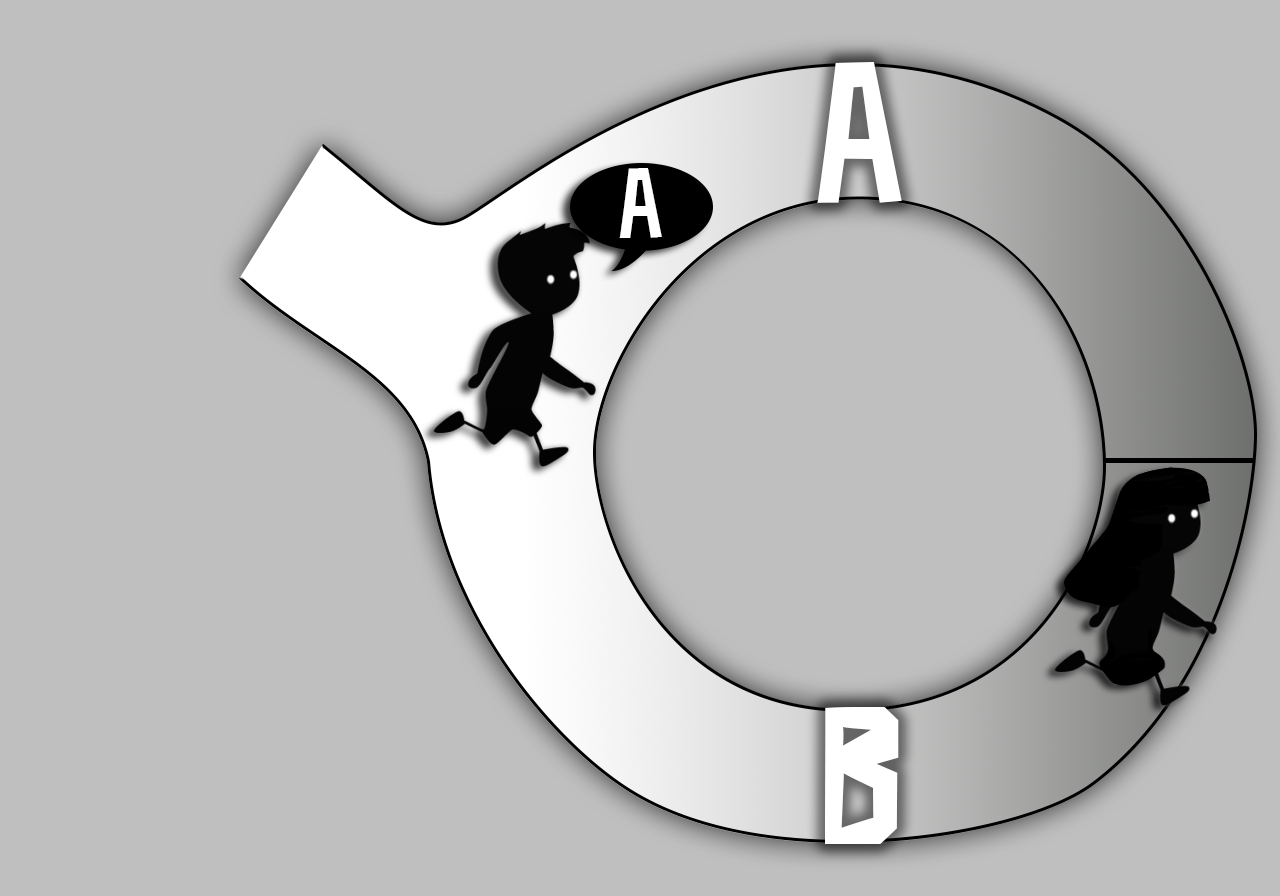
\includegraphics[width=1.\linewidth]{gfx/graficoJL_ZKP_2}\\La cueva. Víctor elige al azar por dónde quiere que regrese Paula.}
	Pero en caso de no conocer la clave, al entrar por uno de los pasillos, tenía una probabilidad del $50\%$ de adivinar cuál pediría Víctor.
	
	
	%\begin{figure}[bth]
	%	\begin{center}
	%		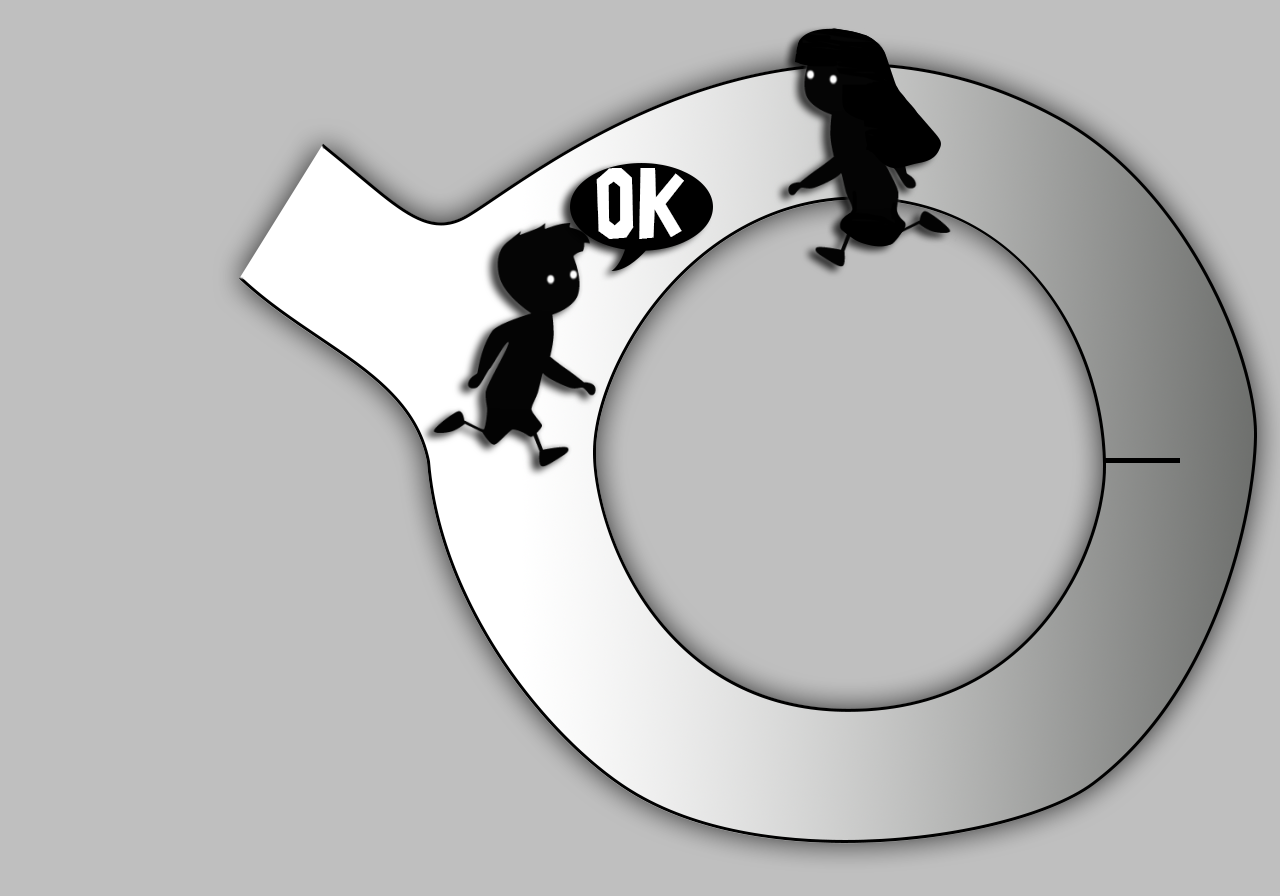
\includegraphics[width=.45\linewidth]{gfx/graficoJL_ZKP_3}
	%	\end{center}
	%	\caption{La cueva. Paula vuelve por el camino pedido.}
	%	\label{fig:ZKPcave3}
	%\end{figure}
	
	Víctor no se queda contento con una sola prueba, pues Paula podría haber tenido suerte, así que la repiten hasta que se convence. Con unas 20 repeticiones, Paula tendría solo una probabilidad de $2^{-20}$, prácticamente nula, de acertar todas las veces y engañar así a Víctor.
	\marginpar{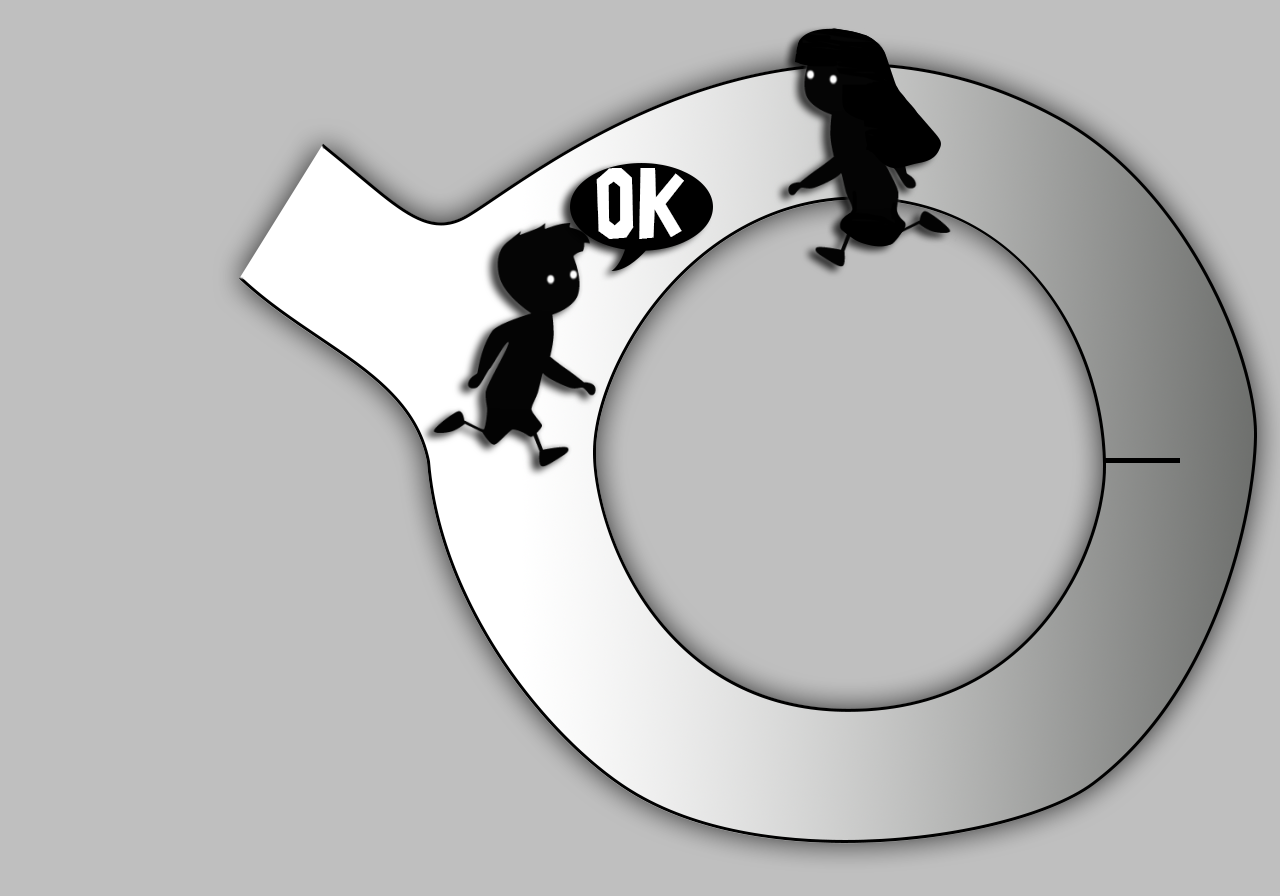
\includegraphics[width=1.\linewidth]{gfx/graficoJL_ZKP_3}\\La cueva. Paula vuelve por el camino pedido.}
	
	
	\textbf{E}va, curiosa de qué hacían Víctor y Paula en la cueva, \textbf{e}spía a Víctor durante todo el proceso. Eva no sabe si Paula y Víctor han acordado previamente qué pasillo pedir por el \textit{walkie-talkie}, y sólo Víctor está seguro de que él los estaba eligiendo al azar y sin previo acuerdo.%, por eso, Eva no puede estar segura de si Paula conoce la clave secreta, o bien estaban \textbf{s}imulando todo para engañarla por cotilla.
	
	Más tarde Eva habla con Víctor, que está seguro de que Paula conoce la clave, y éste querría convencer también a Eva, pero como él no conoce la clave, no puede repetir la prueba a Eva, sólo Paula puede realizarla con éxito.
\end{quote}


\hfil

Utilizando las ZKP, IBM ha desarrollado el protocolo Identity Mixer\footnote{Identity Mixer - \url{https://www.research.ibm.com/labs/zurich/idemix/}}, Idemix para acortar, para autenticación y transferencia de atributos certificados preservando la privacidad. Idemix permite a un usuario autenticarse sin divulgar ningún dato personal. Cada usuario recibe un certificado con múltiples atributos, pero a la hora de presentarlo, pueden decidir qué atributos revelar o de cuáles dar prueba de alguna propiedad, como la de la mayoría de edad, pertenencia a un país de la Unión Europea, etc. De este modo, los datos como su fecha de nacimiento, o país específico no son recopilados y no necesitan ser protegidos, ni procesados por terceros.

\begin{center}
	\textit{``Si tus datos personales nunca son recopilados, no pueden ser robados.''}
\end{center}

Hasta ahora, Idemix o credenciales privadas basadas en atributos han conseguido lidiar con los escenarios típicos de Internet, donde los usuarios pueden autenticarse frente a un proveedor de servicios, demostrando que poseen un credencial válido con permisos, pero sin dar más información. Veremos en el capítulo del estado de arte que las implementaciones actuales están realizadas en Java, lo cual requiere unos recursos mínimos para su ejecución, y, hasta donde llega nuestro conocimiento, este trabajo es la primera propuesta de implementar una solución para la privacidad en IoT, basada en sistemas de credenciales anónimas como Idemix.

\hfil

Como parte de la beca académica de IBM para \textit{Administración de Identidad Preservando la Privacidad aplicada a Internet de las Cosas}, el objetivo de este proyecto es integrar Idemix con el Internet de las Cosas. Para ello nos apoyaremos en el proyecto europeo de ABC4Trust, \ac{P2ABCE}\footnote{P2ABCEngine \url{https://github.com/p2abcengine/p2abcengine}}, que define una arquitectura común, lenguaje y artefactos para unificar distintas soluciones como Idemix de IBM, o U-Prove de Microsoft. Con esto todo dispositivo IoT que lo implemente será compatible con el ecosistema existente.

Una vez los dispositivos pueden ejecutar Idemix, el siguiente paso es utilizar esta herramienta en otros proyectos. Por ejemplo, en un edificio inteligente, distintas políticas de privacidad podrían combinar la protección de los datos recogidos con la seguridad, como el número de personas en el edificio, al termostato sólo le debe interesar si hay más de un mínimo para encender más aparatos de aire acondicionado, pero en caso de incendio, el cuerpo de bomberos puede tener acceso a los datos ocultos por los sensores, para conocer el paradero de las personas atrapadas. Para llegar a soluciones de ese tipo, el primer paso será integrar Idemix en sistemas de gestión de identidad de IoT existentes, como el proyecto FIWARE.

\hfil


\subsection*{Distribución del trabajo}


Este documento se estructura como sigue: En el capítulo \ref{ch:stateoftheart} mostramos el estado del arte mediante la historia de Idemix y trabajos relacionados, analizando los aspectos más interesantes de cara al IoT; luego, en el capítulo \ref{ch:objectives} destacamos los objetivos del proyecto y analizamos en detalle las tecnologías existentes con las que trataremos; en el capítulo \ref{ch:design} describiremos el diseño formal de nuestra solución para IoT e Idemix, y describiremos la implementación de la prueba de concepto; tras esto, en el capítulo \ref{ch:validation} validaremos la implementación y realizaremos tests para comprobar su viabilidad; finalmente, describimos nuestras conclusiones y líneas de trabajo futuro en el capítulo \ref{ch:conclusions}.
